% Bsp. eines Hauptteils

\chapter{Defined Tests for our sensors}
\label{sec:tests}


\section{Infrared Distance Sensor}
\label{sec:TestInfra}

For detailed informations see also \ref{sec:infra} or Data sheet.\\

Infrared Ranging Sensor, intended to measure the distance to ground.

We tested our Infrared Sensor with three different distances: 16cm, 49cm and to the ceiling (which represent the maximum of 150cm). Gathering a lot of data (10 000 values) for each measurement gets a an impression of the jitter and the precision of the value.

In the second steps we did the measurement with different surfaces. They were changing that much, that we search for another possibility to measure the distance. See xxxxxx


\section{Ultrasonic Distance Sensor}
\label{sec:TestUltrasonic}

These tests were only done in theory. Before we finally decided to proceed with that concept, we stoped it.

As we knew that the use of one ultrasonic sensor gives us not that good data and depening of the horizontal angel of the HElikopter, we thought that using three ultrasonic sensors could give us better distance data, independent from the flight angel. But merging 3 sensor to get one good value would a lot of effort and still don't provide us that good data.

While thinking about that concept, we found a better alternative.



\section{LIDAR-lite Laser Distance Sensor}
\label{sec:TestLaser}

For detailed information about the Sensor see also the datasheet or Chapter \ref{sec:laser}.\\

We choose several distances, to validate the measurement. Always taking at least 10 values, to get an impression of the jitter. As the sensor is very good, there is only very small jitter above 20cm.

As the sensor supports distance up to 40 meters, we only tested it with 4 certain distances:\\
very small distance: under 1 meter (0,69m/0,20m)\\
small distance: between 1 and 2 meters (1,46/1,68m)\\
middle distance: above 3 meters ()\\
high distance: above 10 meters ()

Even the measurements diagonal through a room, with a big impact angle, worked really good.\\
Of course we also tested the sensor to different surfaces.


\section{Inertial Measurement Unit (IMU)}

The IMU consists of these 3 sensors:

\subsection{Acceleration and Magnet Sensor(Compass)}

The easiest way to test is, is manually. You trace, gather and display the data from the sensor and do some movements. You can move it as fast as possible over different distances. It should be possible to see at the different curves, how/weather the sensor works.

The Magnet sensor should be tested in a similar way. Depending on the magnetic fields in building, you can display the data and observe how the values change, when you turn the sensor/board/quadrocopter in different directions. In this case it is only relevant in which speed and with which divergence the sensor shows the data. The sensor delivers an absolute value, in which direction your sensor is looking at.


\begin{figure}[H]
	\centering
		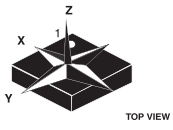
\includegraphics{fig/ch-sensor_testing_concept/compass.png}%[width=1.0\textwidth]
	\label{fig:IMU_com}
	\caption{Compass, Source: Data sheet}
\end{figure}


\subsection{Gyroscope Sensor}

This sensor gives information about the angles of all axis, how the quadrocopter lays in the air.\\
We check the work of sensor with observing the live data, as before.

\begin{figure}[H]
	\centering
		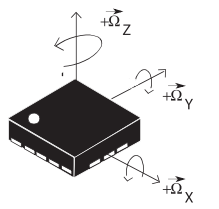
\includegraphics{fig/ch-sensor_testing_concept/gyroscope.png}%[width=1.0\textwidth]
	\label{fig:IMU_Gyro}
	\caption{Gyroscope, Source: Data sheet}
\end{figure}


\begin{figure}[H]
	\centering
		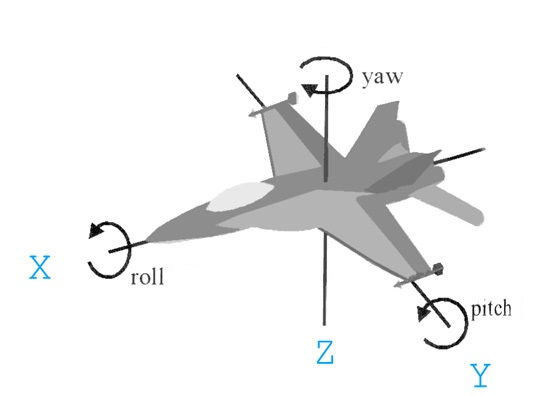
\includegraphics[width=0.7\textwidth]{fig/ch-sensor_testing_concept/timzaman.jpg}%
	\label{fig:IMU_Gyro}
	\caption{Example at plane, Source: timzaman.com}
\end{figure}



\subsection{Pressure Sensor}

This sensor delivers a height compared to the sea level. You can say it is a absolute value.
For that reason it easy to place the sensor at certain heights, and took a lot of data. So we can see the jitter. When lifting it up/down fast for several meters, we can check how fast we get the updated data.

In future this sensor will be controlled with the data form the distance measurements to the ground under us. So we can eliminate the influences from the weather for example.



%\chapter{Realisierung}
%\label{sec:real}
%Beschreibung der HW- und SW-Realisierung
%
%\section{Unter-Kapitel in Realisierung}
%\label{sec:real-unter}
%Beispiel Text
%
%
%\newpage
%\section{Weiteres Unter-Kapitel in Realisierung}
%\label{sec:real-unterWeiter}
%
%\newpage
%\section{Und noch ein Unter-Kapitel in Realisierung}
%\label{sec:real-unterWeiterNoch}
%
%\section{Literaturverweise}
%\label{sec:real-literatur}
%
%Verweise im Text: \cite{doc:stz} und \cite{doc:gun}.
%
%\chapter{Ergebnisse}
%\label{sec:ergeb}
%\enquote{Neuigkeiten} Messergebnisse
